\section{Task 1: Time Series and Correlation Analysis}
\subsection{Results Number Variation Model}
\subsubsection{Exponential Curve Fitting Model}
Observing the results number time series, it's conspicuous that the number experiences a variation that it ascended to its peak and then descended with declining acceleration and persistent fluctuation, which indicated a declining popularity of Wordle Game.

To explain the variation, the results number variation can be divided to two parts:

\begin{itemize}
\item [$\bullet$]Part 1: Gradual and continuous increase of new-coming players.
\item [$\bullet$]Part 2: Players leaving the game or playing the game at lower frequencies.

\end{itemize}

Therefore the results number can be summarized in one formula: 
\begin{align}
    N_{Total}(t)=N_{Uptrend}(t)+N_{Downtrend}(t)
\end{align}
\par For Part 1, the rate of the increase of new-coming players is assumed to be linear proportional to the number of new-coming players:
\begin{align}
    \frac{\mathrm{d}}{\mathrm{d}t}N_{Uptrend}(t)=k_{Up}N_{Uptrend}(t)
\end{align}

Then, $N_{Uptrend}(t)=C_{1}\,e^{k_{1}\,t}$, where $C_{1}$ and $k_{1}$ are constant coefficients.

    


For Part 2, the declining trend of popularity resembled the physical cooling process. Studies have shown that this cooling process could be applied in economics or other fields to describe long term dynamics\cite{article2}. \textbf{Newton's law of cooling} has it that the speed of cooling is proportional to the temperature variation, 
\begin{align}
    \frac{\mathrm{d}}{\mathrm{d}t}N_{Downtrend}(t)=-k_{Down}(N_{Downtrend}(t)-N_{Downtrend}(t_0))
\end{align}

Then $N_{Downtrend}(t)=C_{2}\,e^{k_{2}\,t}$, where $C_{2}$ and $k_{2}$ are constant coefficients.

Therefore, the $N_{Total}(t)$ has the form:
\begin{align}
    N_{Total}(t)=C_{1}\,e^{k_{1}\,t}+C_{2}\,e^{k_{2}\,t}
\end{align}

Fit the curve and then came the results:
\begin{align}
    N_{Total}(t)=544900\,e^{-0.01755\,t}+18760\,e^{0.0007413\,t}
\end{align}

The R-square is 0.9873, which is quite close to 1, suggesting the excellent fitting effect.
\begin{figure}[h]
    \centering
    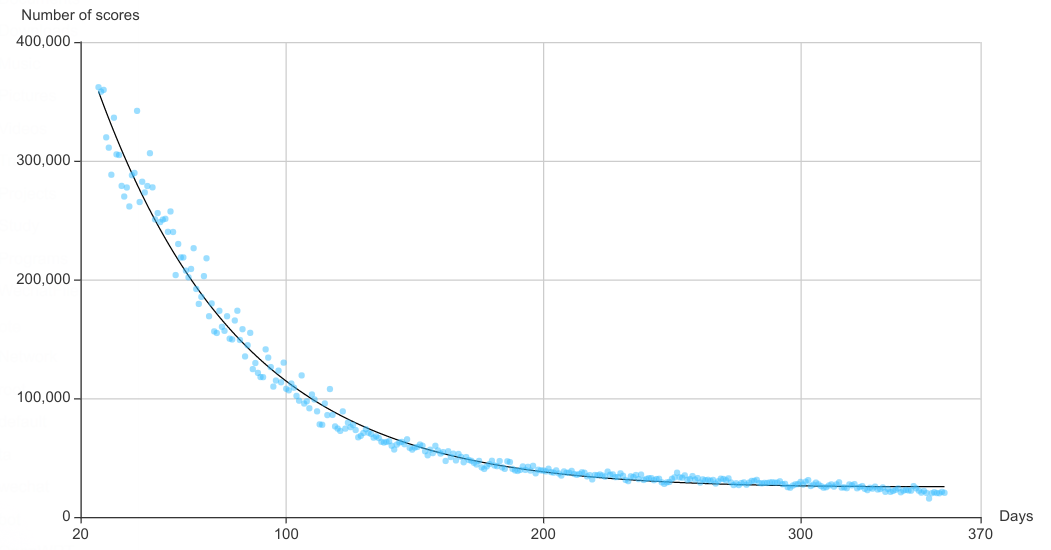
\includegraphics[scale=0.55]{expfit.png}
    \caption{Fitting Curve for Results Number}
    \label{fitting curve}
\end{figure}

\subsubsection{LSTM Prediction Model}
\par The \textbf{exponential fitting curve model} can explain the variation of number of players in a large scale, but the \textbf{smooth curve} it gives leaves out the \textbf{fluctuation information} of data. Therefore, we resorted to LSTM Prediction Model for more practical predictions, since the machine learning algorithm can study the details of fluctuations and flows.

\begin{figure}[h]
    \centering
    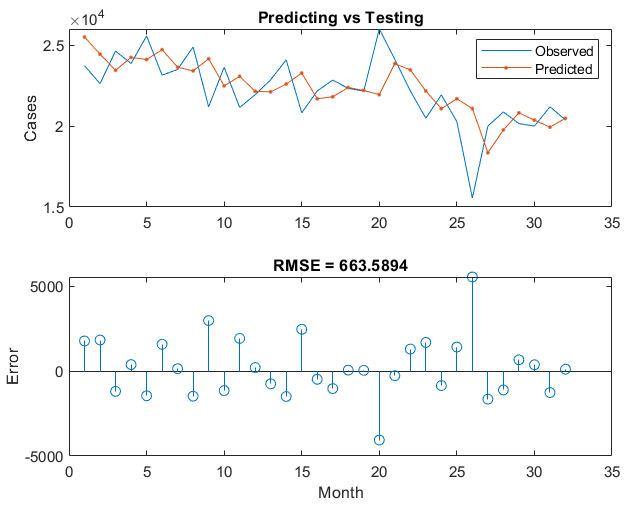
\includegraphics[scale=0.78]{LSTM_total.png}
    \caption{LSTM Prediction: Predicting Results and Testing data}
    \label{LSTM Graph}
\end{figure}

The data of results number was split to $90\%$ training set and $10\%$ testing set. As can be seen from Figure \ref{LSTM Graph}, the predicting results were quite consistent with the testing data, and \textbf{RMSE=663.5894}.

Further predicted the results numbers for next 60 days, and the predicting results number for March 1, 2023 was \textbf{15315}.

Then we applied \textbf{Hypothesis Testing} for calculating the prediction interval at the $\alpha=0.1$ significance level.

\begin{figure}[h]
    \centering
    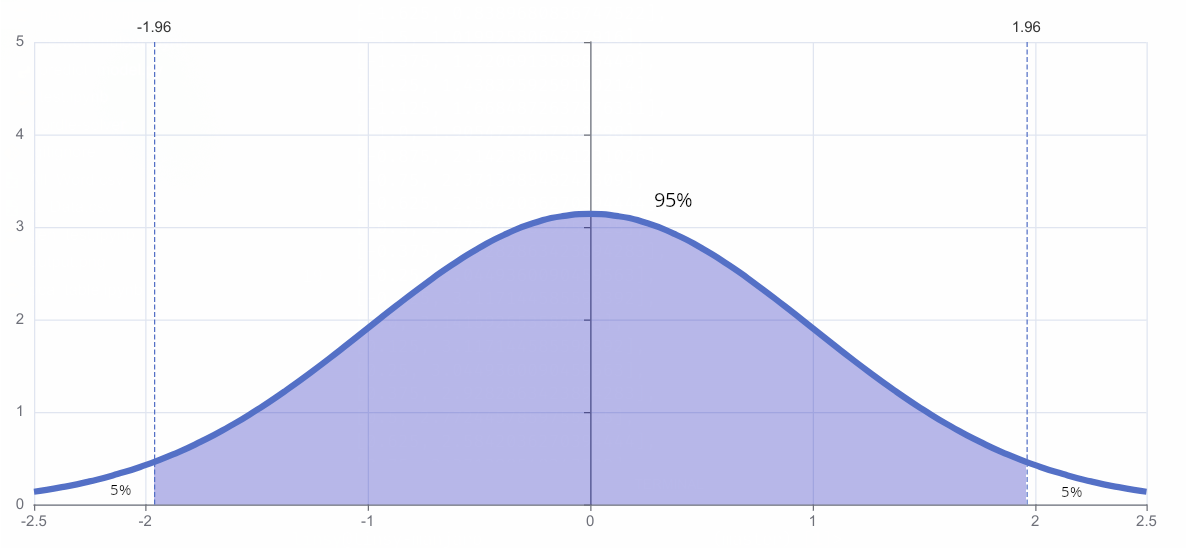
\includegraphics[scale=0.5]{dist.png}
    \caption{Normal Distribution with Labeled Probability}
    \label{norm dist}
\end{figure}

To accept the hypothesis that $N_{Predict}$ is a possible result, $N_{Predict}$ should satisfy the inequality that
\begin{align}
    \phi(|\frac{N_{predict}-15315}{RMSE}|)\leq 97.5\%
\end{align}
where $\phi(x)$ is the PDF for normal distribution, and then
\begin{align}
    |\frac{N_{predict}-15315}{RMSE}|\leq 1.96
\end{align}

Therefore, the prediction interval for $N_{predict}$ is \textbf{[14014,16616]}.

\subsection{Correlation Analysis}
\subsubsection{Word Attributes Model}
In order to explore how \textbf{word attributes} affect the percentage of scores 
played in Hard Mode, we first introduce 4 indications that feature the word. Different words have their own attributes to make them unique. Throughout the paper, we mainly focus on 4 attributes of words that may \textbf{influence players' trial times for guessing}.

\begin{itemize}

    \item [$\bullet$] Vowel Number ($X_{vow}$) : The number of vowels in a word will influence its difficulty to be guessed. Since all words have vowels and there are only five of them among the alphabet, players are more likely to guess words based on them.
    
    \begin{figure}[h]
    \centering
    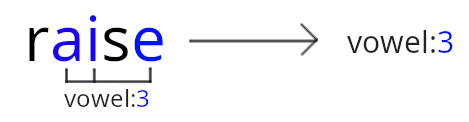
\includegraphics[scale=1.4]{raise.png}
    \caption{Illustration for Vowel Number ($X_{vow}$) }
    \label{norm dist}
    \end{figure}

    \item [$\bullet$] Repetition Number ($X_{rep}$) : Repeated letters appeared in a single word will impact the amount of information it gives out. $X_{rep}$ was calculated by subtracting 1 from highest repetition times for letters in the word.
   
    \begin{figure}[h]
    \centering
    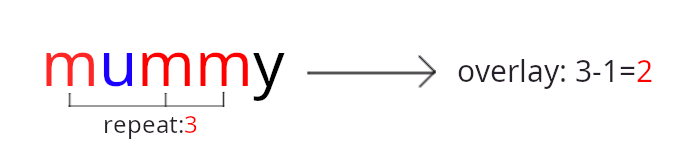
\includegraphics[scale=1.3]{mummy.png}
    \caption{Illustration for Repetition Number ($X_{rep}$) }
    \label{norm dist}
    \end{figure}
    
    \item [$\bullet$] Word Frequency ($X_{freq}$) : The frequency of word used in daily life may directly influence the number of attempts to some extent.
    %%%%%%%%%%%%%%% TODO 词频还需要说什么呀 引用网址
    
    \item [$\bullet$] Information Entropy ($X_{entropy}$) : For this attribute, we learn from the definition of entropy to quantify the information that guessing a certain word can provide. According to Sanderson's algorithm\cite{article3}, the entropy of guessing a word can be represented as the formula:
    %%%%%%%%%%%%%%% TODO 这里需要写成伪代码吗
    
    $$ E[I]=\sum_{x}p(x)\cdot \log_2(\frac{1}{p(x)}) $$
    Where p(x) refers to the probability of each outcome of guessing. For example, if we guess "crane" and the outcome is green on "c" and yellow on "a", the p(x) in this case refers to all possible words that satisfy this constraint divided by the number of all five-letter words in database.
\end{itemize}
\subsubsection{Word Attributes $\&$ Hard-Mode Ratio $X_{ratio}$ Correlation Analysis}
    \par In addition to word attributes, we also need to name a factor to represent the percentage of hard mode scores among all the results. 
    \begin{itemize}
        \item [$\bullet$]
    Hard-Mode Ratio ($X_{ratio}$) : We calculate the value of hard-mode results divided by all the results in a day. Our mission is to use models to find how this ration is related to the word attributes mentioned above.
\end{itemize}

The variables $X_{vow}$,$X_{rep}$,$X_{freq}$,$X_{entropy}$ and $X_{ratio}$ were first normalized to eliminate the influence of units by the z-score formula:
\begin{equation*}
    \Tilde{x}=\frac{x-\mu_{x}}{\sigma_{x}}
\end{equation*}

\par Then we calculated covariance and correlation coefficient to evaluate the overall dependency of every two variables by formulas:

\begin{center}
    Covariance: $\mathrm{Cov}(x,y)=E[(X-E[X])\times (Y-E[Y])]$
\end{center}

\begin{center}
    Correlation Coefficient: $r(x,y)=\dfrac{\mathrm{Cov}(x,y)}{\sigma_x\,\sigma_y}$
\end{center}
\par Then the correlation matrix $R_{word-ratio}$ was generated and shown below.
\par Based on the results shown in the matrix, we find that each covariance of $X_{Ratio}$ with respect to the four word attributes respectively is around 0.1, which indicates that the Hard-Mode ratio are not necessarily affected by word attributes. 

It may be naturally explained by the fact that players won't be influenced by words in-game when selecting game modes before-game.

\subsubsection{Results Distribution Model}
To simplify the distribution of trial times varying between words, based on the abundance of data source and the assumption that the trial times between players are independent and followed a roughly same distribution pattern, we applied \textbf{Central Limit Theorem} and assumed the distribution of trial times to be a \textbf{Gaussian Distribution}.

Therefore, only two variables: \textbf{Mean ($\mu$) and Variance ($\sigma$)} to describe the distribution.

It is worthwhile noticing that the larger Mean ($\mu$) will imply a \textbf{greater difficulty} to guess the word since more trial times are needed.

\subsubsection{Word Attributes and Distribution Correlation Analysis}

\par A covariance matrix was applied again to illustrate the correlation between word attributes and the results distribution.

\par Two conclusions could be reached by the covariance matrix:

(1) The Mean value ($\mu$) is positively correlated to $X_{rep}$, which means that the larger $X_{rep}$ is for a word, the harder it is for players to guess.

\textbf{Possible Explanation:} This coincides with the fact that the more repeated letters a word have, the less probability a player can guess a right letter.

(2) The Mean value ($\mu$) is negatively correlated to $X_{entropy}$, which means that the larger $X_{entropy}$ is for a word, the easier it is for players to guess.

\textbf{Possible Explanation:} The information entropy ($X_{entropy}$) can describe the probability for the word to deduce to other words based on our definition. Correspondingly, it also implies \textbf{how much probability other words can deduce this word}. Therefore, greater information entropy can make the word easier to be guessed,




